\documentclass[a4paper,11pt]{article}
\usepackage[utf8]{inputenc}
\usepackage[T1]{fontenc}
\usepackage[swedish]{babel}
\usepackage{amsmath}
\usepackage{amssymb}
\usepackage{graphicx}
\usepackage{fancyhdr}
\pagestyle{fancy}
\usepackage{a4wide}
\usepackage{anslistings}

\begin{document}
    \title{\textsc{MATLAB} TD}
    \author{Jakob Larsson}
    \date{Oktober 2013}
    \maketitle{}
    \lhead{Jakob Larsson TKDES-1}
    \rhead{\textsc{matlab} inlämming TD Oktober 2013}

    Hej och välkommna till hajk! Idag ska vi prata om inlämmningsuppgifter,
    men inte vilka inlämmningsuppgifter som helst utan en i \textsc{matlab}.

    \section*{Uppgift 1}
    Den här uppgiften finns det inte mycket att säga om.
    \inputmatlabnt{utryck.m}

    \section*{Uppgift 2}
    En funktion baserad  på Heron's formel.
    Funktionen fungerar.

    Paketet \verb+anslistings+ som jag använder för att importera
    \textsc{matlab}-koden
    bråkar lite med strängar som synes. Jag misstänker att \verb+anslistings+
    och \LaTeX har olika uppfattning om vilken teckenuppsättning som används.
    \inputmatlabnt{heron.m}

    \section*{Uppgift 3}
    Plotta tre olika icke triviala funktioner. I figur 3 ser vi graferna.
    Koden för det tre plottarna är väldigt lika, det skulle nog att gå att bryta
    ut till en gemensam funktion.
    \inputmatlabnt{ex3.m}
    \begin{figure}
        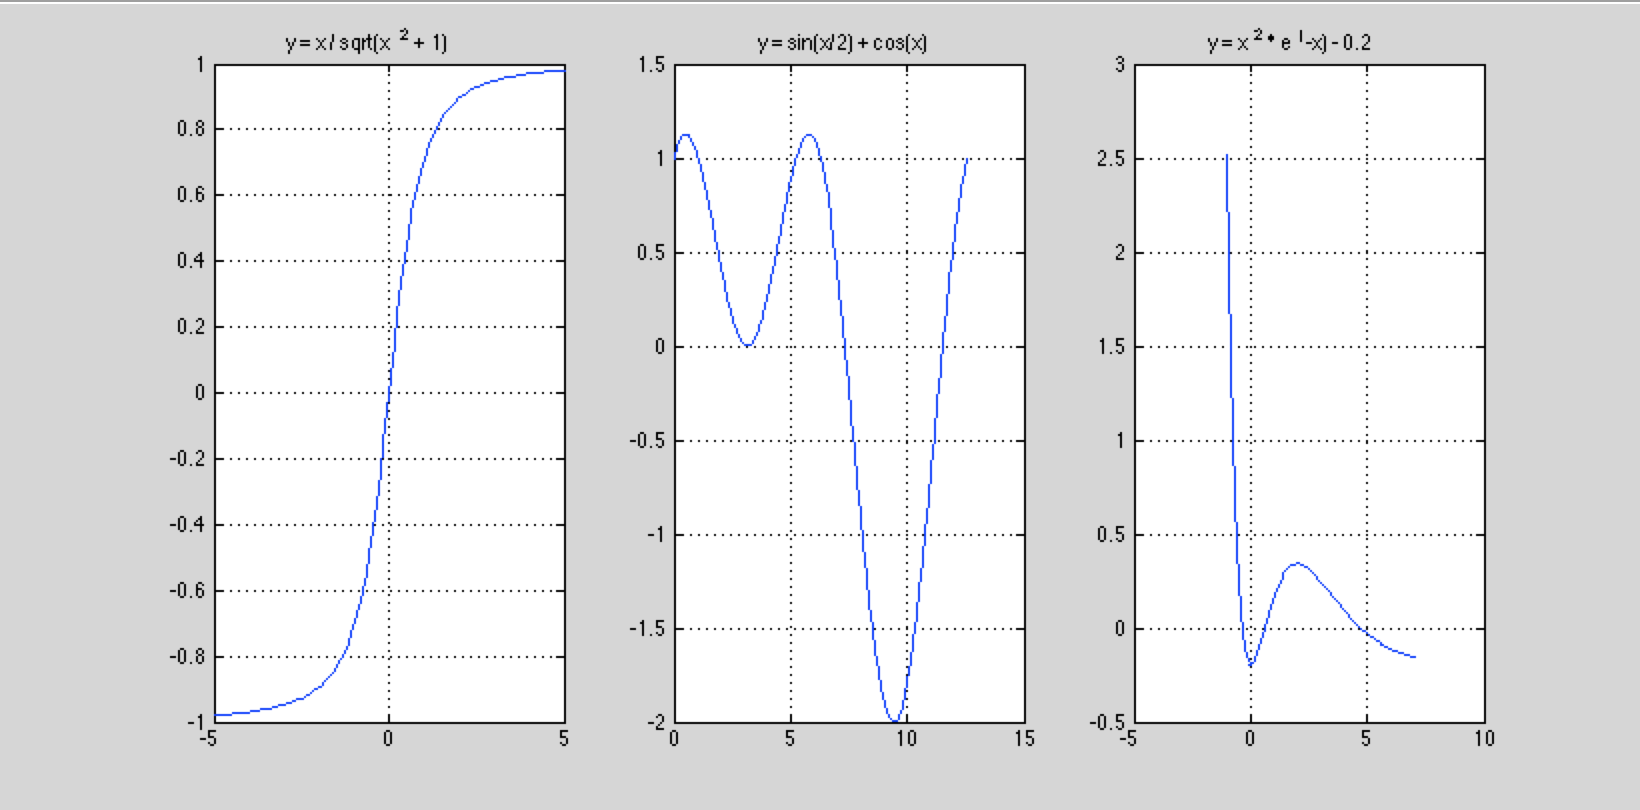
\includegraphics[width=\textwidth]{ex3.png}
        \caption{Snygga grafer}
    \end{figure}

    \section*{Uppgift 4}
    \subsection*{a)}
    Det var något oklart först att man skulle använda \verb=meshgird=.
    Men när man tillslut förstår hur den funktionen funkar är resten simpel.
    \begin{figure}
        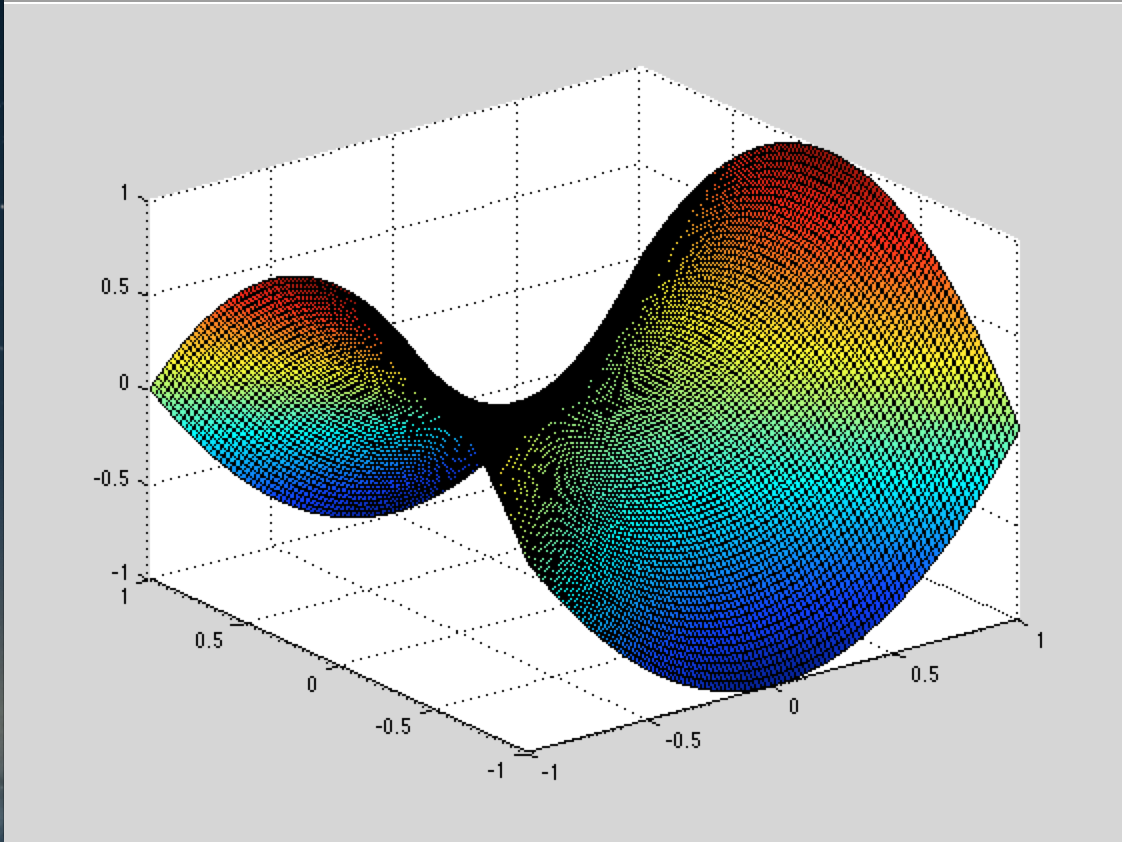
\includegraphics[width=\textwidth]{ex4a.png}
        \caption{Sadelyta i färg}
    \end{figure}
    \inputmatlabnt{ex4a.m}

    \subsection*{b)}
    \begin{figure}
        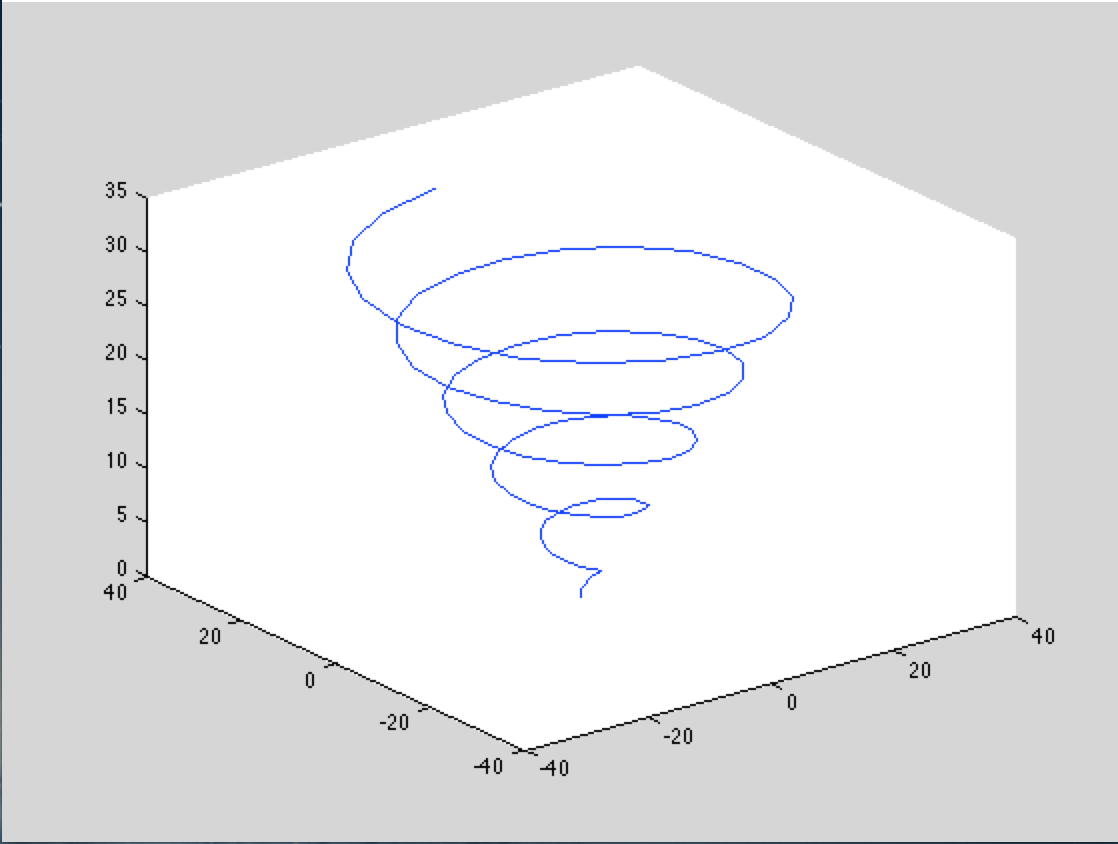
\includegraphics[width=\textwidth]{ex4b.png}
        \caption{Konisk spiral}
    \end{figure}
    Den här uppgiften var mer rättfram, att plotta i tre dimensioner fungerar
    precis som i två med \textsc{matlab}.
    \inputmatlabnt{ex4b.m}

    \section*{Uppgift 5}
    \begin{figure}
        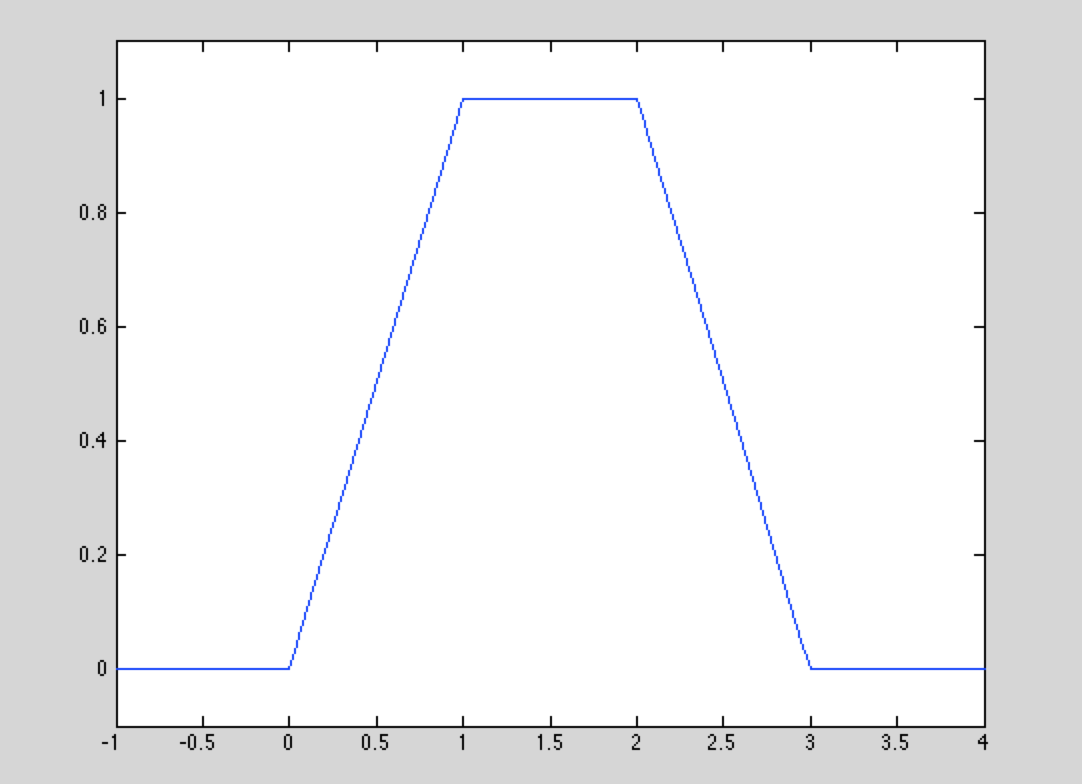
\includegraphics[width=\textwidth]{ex5.png}
        \caption{funk5}
    \end{figure}
    \inputmatlabnt{funk5.m}
    \inputmatlabnt{ex5b.m}
    I Figur 5 ser vi den lite speciella \verb+funk5+.

    \section*{Uppgift 6}
    En rekursivt definerad funktion som ger tal $n$ i Fibonaccis talföljd.
    Tillskillnad från den naiva implementationen kör denna funktion på
    $\mathcal{O}(n)$.
    I teorin är funktionen \verb+fibonacci+ definerad för $n \in \mathbb{Z}_+ $.
    Dock så tillåter \textsc{matlab} enbart rekursion till ett maximalt djup.
    Som standard är det maximala djupet satt till 500.
    Det betyder att \verb+fibonacci+ i praktiken oftast är definerad endast för
    $n \in \left\{ 1...499 \right\}$.
    \inputmatlabnt{fibonacci.m}

    \section*{Uppgift 7}
    \begin{figure}
        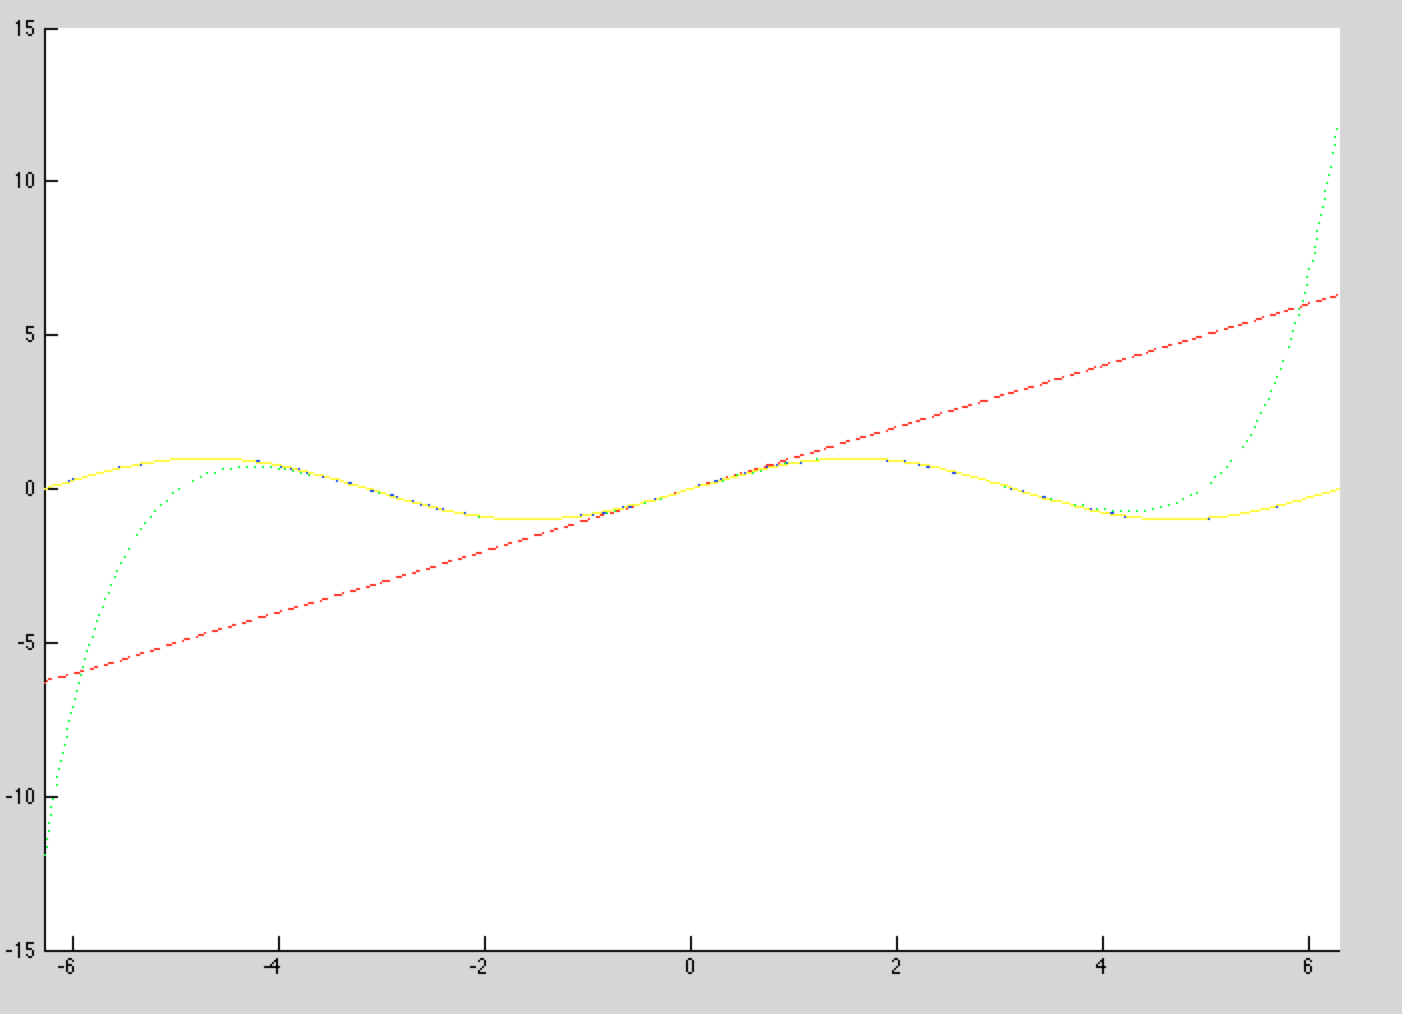
\includegraphics[width=\textwidth]{ex7.png}
        \caption{Approx. av sinus}
    \end{figure}
    Uppgiften är att skriva en funktion som beräknar en faklaurin-utveckling för
    $\sin (x)$.

    \inputmatlabnt{funk7.m}

    En sådan funktion följer att väldigt vanlig mönster:
    \begin{enumerate}
        \item Ta en lista/vektor/följd av heltal.
        \item Applicera en funktion på nämnda lista.
        \item Summera.
    \end{enumerate}
    Så jag valde att skriva funktionen \verb+fsum+ som gör just detta.
    funktionen i sig är väldigt kort, det är i princip bara rad 10. Resten finns
    för att ge lite felxibilitet i vilka argument funktionen tar.
    \inputmatlabnt{fsum.m}
    I figur 5 kan man se resultatet. Det är lite svårt att urskilja de olika
    funktionerna i grafen. Den utveckling med 100 termer går inte att skilja
    från $\sin (x)$ på detta intervall.
    \inputmatlabnt{test7.m}

    \section*{Uppgift 8}
    I uppgiften var det specifierat att man skulle inplementera Bubblesort,
    men de kändes tråkigt. Så här följer istället den mycket coolare Quicksort
     som i genomsnitt kör på
    $\mathcal{O}(n \log(n))$.
    Eftersom min implementation här är rekursiv kommer den inte att klara
    vektorer över en viss storlek pga. \textsc{matlab}s rekursions-max.
    I teorin finns dock inget som begränsar funktionen då rekursionssteget
    är det sista som händer i funktionen.
    \footnote{en.wikipedia.org/wiki/Tail\_call}
    \inputmatlabnt{minsort.m}

\end{document}
